% Lecture for ph2a Caltech 2017: Vibrations and Waves
\documentclass[pdf,handout, hideothersubsections]{beamer}
\usepackage{beamerthemeshadow}
\mode<presentation>
  {
    \usefonttheme{structuresmallcapsserif}
    \usetheme{CambridgeUS}
    \usecolortheme{seahorse}
    %\useinnertheme{circles}
%    \useoutertheme{tree}
  }

\usepackage{svg}
\usepackage{xmpmulti}
\usepackage{mathtools}
%\usepackage{enumitem}
\usepackage{hyperref}
\hypersetup{
    pdffitwindow=true,     % window fit to page when opened
    colorlinks=true,       % false: boxed links; true: colored links
    linkcolor=orange,      % color of internal links 
    citecolor=green,       % color of links to bibliography
    filecolor=magenta,     % color of file links
    urlcolor=blue,         % color of external links
    pdfstartview={Fit}
}

% Fonts/encoding
\renewcommand{\UrlFont}{\tiny}
\usepackage[utf8]{inputenc}
\usepackage[T1]{fontenc}
%\usepackage[sc,medium,raggedright]{titlesec}
\usepackage{newtxmath}
%\usepackage{libertine}
\usepackage[osf]{ebgaramond}

\graphicspath{{Figures/}}

\begin{document}
\title{Normal Modes}  
\author{Caltech: ph2a}
\date{12 - Oct - 2017}


\frame{\titlepage} 

\frame{\frametitle{Table of contents}\tableofcontents} 

\setbeamerfont{footnote}{size=\tiny}

\section{Previous Summary}
\begin{frame}
\frametitle{Last Time:}
\begin{itemize}
\item Coupled oscillators have multiple free vibration frequencies/modes.
\item These free oscillation frequencies are called eigenfrequencies.
\item The oscillation functions are the eigenfunctions.
\item Linear algebra can be used to solve for these functions.
\end{itemize}
\end{frame}


\begin{frame}
\frametitle{Properties of Modes in Coupled Osc.}
\begin{enumerate}
\pause
\item $\omega_{1,i}=\omega_{2,i}=\omega_i$~(for the i$^{th}$ mode)
\pause
\item $A_{1,i}, A_{2,i} \ne f(t)$; i.e. amplitudes are constant
\pause
\item A's are constant, so the relative phases of the modes are
  constant.
\pause
\item \underline{Stable}: w/o friction the oscillations go on
  forever. There is no mixing of energy \emph{between} eigenmodes
\pause
\item \textbf{Complete}: Any free oscillation can be decomposed into a sum of
  normal modes.

\end{enumerate}
\end{frame}



\section{Coupled Oscillator}
\begin{frame}
\frametitle{Coupled Oscillators: Overview}
\pause
\begin{enumerate}
\item For free vibrations, $m \ddot{x} + b \dot{x} + k x = 0$.
\pause
\item In a coupled systems, there can be several springs and several
  masses with many inter-connections.
\pause
\item Can be used for analysis of many kinds of linear systems.
\pause
\item Matrix methods are very handy in solving systems of coupled
  differential equations: linear algebra is useful for solving systems
  of linear equations.
\end{enumerate}
\end{frame}

\subsection{Examples}
\begin{frame}
\frametitle{Examples}

\begin{itemize}
\item 2 masses, 3 springs (Airtrack Demo) \\
\url{https://www.myphysicslab.com/springs/double-spring-en.html} \\
\url{http://www.falstad.com/coupled/}
%\pause
\item 2 Pendula coupled by a weak spring
%\pause
\item Double Pendulum (python demo) \\
\url{https://www.myphysicslab.com/pendulum/double-pendulum-en.html}


\end{itemize}


\end{frame}



\subsection{Equations of Motion}


\begin{frame}
\frametitle{Summary of the EigenMode analysis:}
\begin{enumerate}
\item Make a diagram of the system. Draw the forces.
\pause
\item Write down the differential eqs. for the forces (e.g. 
$\ddot{x} = -\frac{k}{m} x$)
\pause
\item Write down the initial guess for the solutions,
  e.g. $\tilde{x}_k = \tilde{A}_k e^{i \omega t}$
\pause
\item Plug guesses into diff. eqs. Re-arrange so it `looks easy' to put
  into matrix form.
\pause
\item Write as a matrix equation (with $N = $ number of modes): \\
($N \times N$ matrix) $\times$ ($N \times 1$ column vector) = 0
\pause
\item Set the determinant of the $N \times N$ matrix = zero to find
  the eigenvalues (solve for the possible values of $\omega$)
\pause
\item Plug the eigenvalues back into the matrix equation to solve for
  the complex amplitudes, $\tilde{A}_k$
\end{enumerate}
\end{frame}


\begin{frame}
\frametitle{Two Masses + Three Springs}
\begin{columns}

  \begin{column}{0.5\textwidth}
\pause
    \includegraphics[width=0.85\textwidth]{2masses3springs.jpg}
\begin{itemize}
\item $k_1 = k_2 = k_3 = k$
\item $m_1 = m_2 = m$
\end{itemize}
  \end{column}

  \begin{column}{0.5\textwidth}
    \pause
    Forces on Mass 1:
    \begin{equation}
      F_1 = m \ddot{x_1} = -k x_1 + k (x_2 - x_1)
    \end{equation}
    \pause
    Forces on Mass 2:
    \begin{equation}
      F_2 = m \ddot{x_2} = -k x_2 - k (x_2 - x_1)
    \end{equation}
    \pause
    2 Eqs \& 2 Unknowns:
    \begin{align}
      m \ddot{x_1} + 2 k x_1 - k x_2 &= 0 \\
      m \ddot{x_2} + 2 k x_2 - k x_1 &= 0
    \end{align}
  \end{column}

\end{columns}
\end{frame}



\begin{frame}
\frametitle{Two Masses + Three Springs}
    \pause
\begin{enumerate}
\item For SHO, we guessed $\tilde{x} = A e^{i (\omega t + \phi_0)}$
\pause
\item For CHO, we use $\tilde{x_1} = A_1 e^{i \omega t}$ and
  $\tilde{x_2} = A_2 e^{i \omega t}$; assuming $A_1$ and $A_2$ are complex.
\pause
\item Plugging into Eqs. 3 \& 4, we get: \\
\begin{align*}
\Big[ -\omega^2 A_1 + 2 \frac{k}{m}A_1 - \frac{k}{m}A_2 \Big] e^{i
  \omega t} &= 0 \\
\Big[ -\omega^2 A_2 + 2 \frac{k}{m}A_2 - \frac{k}{m}A_1 \Big] e^{i
  \omega t} &= 0
\end{align*}
\pause
\item Divide both sides by $e^{i \omega t}$ and using $\omega_0^2 =
  k/m$, we get:
\pause
\begin{align*}
\Big[ -\omega^2 A_1 + 2 \omega_0^2 A_1 - \omega_0^2 A_2 \Big] &= 0 \\
\Big[ -\omega^2 A_2 + 2 \omega_0^2 A_2 - \omega_0^2 A_1 \Big] &= 0
\end{align*}

\end{enumerate}
\end{frame}

\section{Eigenfrequencies}
\begin{frame}
\frametitle{Matrix Methods: Eigenvalues}
\pause
Rewrite in matrix form to allow using linear algebra: \\
\[
\begin{bmatrix}
-\omega^2 + 2 \omega_0^2 & -\omega_0^2 \\
-\omega_0^2 & -\omega^2 + 2 \omega_0^2
\end{bmatrix}
\begin{bmatrix}
A_1 \\
A_2
\end{bmatrix}
=
\begin{bmatrix}
0 \\
0
\end{bmatrix}
\]
\pause
which we can write as
\[
M_{j k} 
\begin{bmatrix}
A_1 \\
A_2
\end{bmatrix}
=
\begin{bmatrix}
0 \\
0
\end{bmatrix}
\]
\pause
Multiplying through by the inverse matrix, $M_{jk}^{-1}$, we get
\[
M_{jk}^{-1} M_{j k} 
\begin{bmatrix}
A_1 \\
A_2
\end{bmatrix}
=
M_{jk}^{-1}
\begin{bmatrix}
0 \\
0
\end{bmatrix}
\]
\pause
which just means $A_1 = 0$ and $A_2 = 0$, which is the trivial
solution of no motion of the oscillators. 
\pause
The only cases in which
this is not true, are the ones for which \textcolor{blue}{the matrix inverse,
$M_{jk}^{-1}$, \emph{does not exist}}.

\end{frame}


\begin{frame}
From linear algebra, we remember that the non-invertible matrices have
a determinant equal to zero:
\[
\begin{vmatrix}
-\omega^2 + 2 \omega_0^2 & -\omega_0^2 \\
-\omega_0^2 & -\omega^2 + 2 \omega_0^2
\end{vmatrix}
= 0
\]
\pause
which gives us the following quadratic equation:
\pause
$(-\omega^2 + 2 \omega_0^2)^2 -\omega_0^4 = 0$ \\
\pause
and solving for $\omega$, we have
\centering
\pause
$\omega^2 = 2 \omega_0^2 \pm \omega_0^2$ \\
\pause
so $\omega = (\omega_0, \sqrt{3} \omega_0)$

\end{frame}










\section{Eigenmodes}
\begin{frame}
\frametitle{Eigen (Normal) Modes}
\pause
Plugging the eigenfrequencies back into our equations, we get:
\pause
\begin{align}
\omega = \omega_0 :  -\omega_0^2 A_1 + 2 \omega_0^2 A_1 - \omega_0^2 A_2 &=
0 \implies A_1 = A_2\\
\omega = \sqrt{3} \omega_0 :  -\omega_0^2 A_1 - 3 \omega_0^2 A_2 + 2 \omega_0^2 A_2 &=
0 \implies A_1 = - A_2
\end{align}
\pause
These are the \emph{symmetric} and \emph{anti-symmetric} solutions,
respectively:

\begin{block}{Symmetric Mode:}
$ \tilde{x}_1 = \tilde{C}_+ e^{i \omega_0 t}, \tilde{x}_2 = \tilde{C}_+
e^{i \omega_0 t}$
\end{block}
\begin{alertblock}{Anti-Symmetric:}
$\tilde{x}_1 = \tilde{C}_- e^{i \sqrt{3} \omega_0 t},
\tilde{x}_2 = -\tilde{C}_- e^{i \sqrt{3} \omega_0 t}$
\end{alertblock}

\end{frame}

\section{Torsionally Coupled Pendula}
\begin{frame}
\frametitle{Example: Weakly Coupled Pendula}

\begin{columns}
  \begin{column}{0.3\textwidth}
    \includegraphics[width=4cm]{TorsionCoupled.png}
  \end{column}
  \pause

\begingroup
\footnotesize
  \begin{column}{0.7\textwidth}
Two pendula pivot about an axis, $A$, and are constrained to rotate in
a plane perpendicular to that axis. The pivot points are fixed. The
pendula are coupled by a weak torsional spring that obey's Hooke's law
with a torsional spring constant, $\kappa$.:
\begin{equation*}
\tau = \kappa (\theta_1 - \theta_2)
\end{equation*}
\pause

\begin{enumerate}
\item (2.5 pts) Write the coupled diff. eq. describing the motion of
  the pendula for $\theta_n << 1$.

\item (2.5 pts) Find the two eigenfreqencies.

\item (2.5 pts) Find the two eigenfunctions. The overall complex
  amplitude for each eigenfunction should remain undetermined.

\item (2.5 pts) Determine the time evolution of each pendulum with the
  initial conditions $\theta_1(0) = 0$ and $\theta_2(0) = A$, and both
  starting with zero velocity. Sketch the functions for at least 2
  cycles. Assume that $\kappa = \frac{1}{8} m g L$.

\end{enumerate}

\end{column}
\endgroup
\end{columns}
\end{frame}

\begingroup
\footnotesize
\begin{frame}
\frametitle{Part 1}
\begin{columns}[T]

  \begin{column}{0.3\textwidth}
     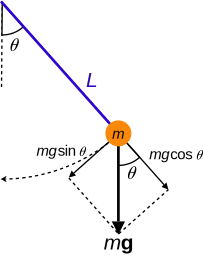
\includegraphics[width=\textwidth]{Simple_pendulum_generalized_coordinates.pdf}

  \end{column}
\pause
  \begin{column}{0.7\textwidth}
  \begin{enumerate}
  \item Motion of pendulum is \emph{rotational}, not translational, so instead of $F = m a$, use $\tau = I \ddot{\theta}$, where $\tau$ is the torque, and $\theta$ is the angle of the pendulum wire. \\
    \pause
  \item   
    \begin{align*}
      I \ddot{\theta}_1 &= \vec{r} \times \vec{F} \\
      m L^2 \ddot{\theta}_1 &= -m g L \sin{\theta_1} \\
      m L^2 \ddot{\theta}_1 &\simeq -m g L \theta_1
    \end{align*}
   \pause
   \item And we also add our weak torsional spring's torque:
\begin{align}
 m L^2 \ddot{\theta}_1 &= -m g L \theta_1 - \kappa (\theta_1 -
                         \theta_2) \label{eq:tor1}\\
 m L^2 \ddot{\theta}_2 &= -m g L \theta_2 + \kappa (\theta_1 -
     \theta_2) \label{eq:tor2}
\end{align}
Using the same logic for the second pendulum, while being careful
about the sign of the coupling torque.     

  \end{enumerate}

  \end{column}

\end{columns}

\end{frame}
\endgroup

\begingroup
\footnotesize
\begin{frame}
\frametitle{Part 2}
\begin{enumerate}
\item Use the usual initial guesses: $\tilde{\theta}_k = \tilde{A}_k
  e^{i \omega t}$
\item Plugging in to \eqref{eq:tor1}, and \eqref{eq:tor2}, and dividing by $e^{i \omega t}$, we get:
\begin{align}
 -m L^2 \omega^2 A_1 &= -m g L A_1 - \kappa (A_1 - A_2) \\
 -m L^2 \omega^2 A_2 &= -m g L A_2 + \kappa (A_1 - A_2)
\end{align}
\item Dividing by $m L^2$ and regrouping:
\begin{align}
 \omega^2 A_1 - \omega_0^2 A_1 + \frac{\kappa}{m L^2} (A_1 - A_2) &= 0 \\
 \omega^2 A_2 - \omega_0^2 A_1 - \frac{\kappa}{m L^2} (A_1 - A_2) &= 0
\end{align}

\end{enumerate}
\end{frame}
\endgroup

\begingroup
\footnotesize
\begin{frame}
\frametitle{Part 2b}

Now we can write it as a matrix equation (setting $ \frac{\kappa}{m
  L^2} = \omega_T^2$ :
\[
\begin{bmatrix}
\omega^2 - \omega_0^2 + \omega_T^2 & -\omega_T^2 \\
-\omega_0^2 - \omega_T^2 & \omega^2 + \omega_T^2
\end{bmatrix}
\begin{bmatrix}
A_1 \\
A_2
\end{bmatrix}
=
\begin{bmatrix}
0 \\
0
\end{bmatrix}
\]
\pause
Setting the determinant equal to zero:
\begin{align}
(\omega^2 + \omega_T^2)(\omega^2 - \omega_0^2 + \omega_T^2) -
  (-\omega_T^2)(-\omega_0^2 - \omega_T^2) = 0
\end{align}
we can algebraically solve for $\omega$ in terms of $\omega_0$ and $\omega_T$.
\end{frame}
\endgroup

\begin{frame}
\frametitle{Part 3}
Plug the eigenfrequencies back into Eqs 11 \& 12 to solve for the
(complex) values of $A_1$ and $A_2$.

\end{frame}


\begin{frame}
\frametitle{Part 4: Initial Conditions}
Solve for the relative phases and amplitudes of $A_n$ by using the
initial conditions on $\theta_n(0)$ and $\dot{\theta_n}(0)$

\end{frame}

% \section{Beats}
% \begin{frame}
%  \frametitle{Beats: Examples}


% \end{frame}




% \section{Summary}
% \begin{frame}
% \frametitle{Modes in Coupled Oscillators}
% \begin{enumerate}
% \pause
% \item $\omega_{1,i}=\omega_{2,i}=\omega_i$~(for the i$^{th}$ mode)
% \pause
% \item $A_{1,i}, A_{2,i} \ne f(t)$; i.e. amplitudes are constant
% \pause
% \item A's are constant, so the relative phases of the modes are
%   constant
% \pause
% \item \underline{Stable}: w/o friction the oscillations go on forever
% \pause
% \item \textbf{Complete}: Any motion can be decomposed into a sum of
%   normal modes.

% \end{enumerate}
% \end{frame}


\end{document}

